\section{Passive-Aggressive algorithm with Bandit feedback for multilabel classification}
\label{sec:BPAS}
Before introduce this algorithm, let's get some notations and preliminaries. It is applied in a sequence of consecutive rounds. On round $t$, the learner is given an instance vector $\xt\in\mathscr{X}$ and outputs a binary vector $\hY\in \{0,1\}^K$ representing a label subset from the set of all labels. In the general setting, the true response $Y_t\in\{0,1\}^K$ associated with $\xt$ is generated after the prediction. In the bandit setting, the learner can not observe $Y_t$, only receive $\beta_t\in\{0,\frac{1}{2},1\}^K$ as partial feedback, where for $\forall k\in\{1,\dots,K\}$:
\begin{equation}
\beta_t^k = \left\{\begin{matrix}
1 			& \hy^k = y_t^k = 1 \\
0 			& \hy^k = 1 \& y_t^k = 0 \\
\frac{1}{2} & \hy^k = 0
\end{matrix}
\right.
\end{equation}
The widely known Binary relevance Method(BM) \cite{read2008pruned} transfers the multi-label task into  several single independent binary classification tasks for each label. BM approach is theoretically simple and intuitive. Its assumption of label independence makes it ignores label correlations that exist in the training data. The most important advantage of BM is its low computational complexity compared to other methods.

We consider a multilabel classification model $\mathbf{f(x)}$ is a mapping function $\mathscr{X}\rightarrow \{0,1\}^K$. The output of the model is a binary vector:
\[\mathbf{h(x)} = (h_1(\mathbf{x}),\dots,h_K(\mathbf{x}))\]
here $\mathbf{h(x)}$ is taken from a class of hypothesis $\mathbf{H}$ parameterized by a $K\times d$ matrix of real weights $W$. Hence, $\forall i\in [K]. h_i(\mathscr{x}):= \frac{1}{2}(1+sign<W^i,x>)$ where $W^i$ is the $i^{th}$ row of $W$. If the score $<W^i,x>$ is positive, the prediction is $\hat{y}_t^i = 1$, else it equals $0$.

The algorithm BPA is based on the online Passive-Aggressive approach. Consistently with paper~\cite{crammer2006online}'s writing, a feature function: $\Phi(x,i)$ is a $K\times d$ matrix which is composed of $K$ features vectors of size $d$. All rows of $\Phi(x,i)$ are zero except the $i^{th}$ row which is set to $x$. It can be remarked that $<\Phi(x,i),\Phi(x,j)> = \parallel{x}\parallel^2$ if $i=j$ and $0$ otherwise. In our case, $<W,\Phi(x,i)>$ is equal to $<W^i,x>$.

In the bandit setting, a strategy needs to be set to address the exploration/exploitation trade off. In this paper, we use the strategy $\epsilon$-greedy in Section~\ref{sec:greedy}. At each round $t=1,2,\dots$ the algorithm selects a subset $\tilde{Y}_t$ according to the probabilities $P_t = \left(P(\tilde{y}_t^1) = 1| \hat{y}_t^1,\dots, P(\tilde{y}_t^K = 1|\hat{y}_t^K)\right)$, with:
\begin{equation}
\label{equa:epsilongreedyml}
p(\tilde{y}_t^i = 1|\hat{y}_t^i) = (1-\epsilon)\cdot \1_{(\hat{y}_t^i=1)}+ \epsilon\cdot\frac{\sum_{k=1}^{K}\1_{(\hat{y}_t^k = 1)}}{K}
\end{equation}

Let the cardinality of $\hat{Y}$ be noted $Card(\hat{Y}) = \sum_{k=1}^{K}\1_{(\hat{y}^k = 1)}$.
\begin{lema}
With the notations introduced so far, when following an $\epsilon$-greedy random selection, the expected cardinality of $\tilde{Y}_t$ is equal to $Card(\hat{Y}_t)$.
\end{lema}
\begin{proof}
\[\E[Card(\tY)] = \sumk P(\ty^k = 1| \hy^k)\]
\[\E[Card(\hY)] = (1-\epsilon)\sumk \1_{\hy^k = 1}+\epsilon \sumk \1_{\hy^k = 1}\]
\[\E[Card(\tY)] = \sumk\1_{\hy^k = 1} = Card(\hY)\]
\end{proof}

The instantaneous loss is defined as a piece-wise hinge loss function $L_t = \sum_{k=1}^{K} l_t^k$, where
\begin{equation}
\label{eq:loss}
l_t^k = [\mathds{1}_{ \tilde{y}_t^k = 1} + \left(1-2\beta_t^k\right) \left\langle W, \Phi(x_t,k)\right\rangle]_{+}
\end{equation}
with $1-2\beta_t^i$ equals to $-1$ when $\tilde{y}_t^i=y_t^i=1$,  $+1$ when $\tilde{y}_t^i = 1\ \&\ y_t^i = 0$ and $0$ otherwise (see Algorithm~\ref{algo:BPAml}). This loss is the standard hinge loss $[1-\left\langle W,\Phi(x_t,\tilde{y}_t)\right\rangle]_{+}$ when the prediction is positive correct: it stays at $0$ for $\left\langle W,\Phi(x_t,\tilde{y}_t)\right\rangle \geqslant 1$ and then increases for decreasing values of $\left\langle W,\Phi(x_t,\tilde{y}_t)\right\rangle$. In contrast, when the prediction is positive incorrect, the loss is equal to $[1+\left\langle W,\Phi(x_t,\tilde{y}_t)\right\rangle]_{+}$, i.e., stays at $0$ for $\left\langle W,\Phi(x_t,\tilde{y}_t)\right\rangle \leq 1$ and then increases for increasing values of $\left\langle W,\Phi(x_t,\tilde{y}_t)\right\rangle$. For the negative prediction $\tilde{y}_t^i = 0$, the loss equals to $0$.

In this section, we introduce a novel online learning algorithm (see algorithm ~\ref{algo:BPAml}), which is a variant of the Online Passive-Aggressive algorithm adapted to the multi-label classification in the bandit setting. It is named BPAs (Bandit Passive-Aggressive with multiple labels).

The goal of online learning is to minimize the cumulative loss for a certain prediction task from  sequentially arriving training samples.  Online Passive-Aggressive achieves this goal by updating some parameterized model $W$ in an online manner with the instantaneous losses from the arriving data $x_{t}$ and corresponding responses $y_{t}$, with $t\geqslant 0$. The loss $l(W;(x_t,y_t))$ can be the hinge loss. The solution will be derived from the optimization problem:
\begin{equation}
\begin{split}
\label{eq:update}
W_{t+1} = \underset{W\in \mathbb{R}^{K\times d}}{argmin}\frac{1}{2}\parallel{W-W_t}\parallel^2 \\ 
s.t.\ l_t\left(W;(x_t,y_t)\right)=0
\end{split}
\end{equation}

Intuitively, if $W_t$ suffers no loss from new data, i.e., $l\left(W;(x_t,y_t)\right) = 0$, the algorithm passively assigns $W_{t+1} = W_t$; otherwise, it aggressively projects $W_t$ to the feasible zone of parameter vectors that attain zero loss. 

Similarly to Online Passive-Aggressive, we output at each round  a subset prediction $\hat{Y}_t \in \{0,1\}^K $ %with the scores of $\left\langle W_t, x_t\right\rangle$,
according to the binary prediction as following:
\[\hat{y}_t^i = \text{sign}(<W,\Phi(x,i)>)\]
%Unlike the conventional supervised learning paradigm, the optimal solution is directly . 
Then an $\epsilon$-greedy exploration is performed, where $\tilde{Y}_t\in \{0,1\}^K$ is the result of a random draw from  $\mathbf{P}_t$ (see Eq.(\ref{equa:epsilongreedyml})).

The linear classifiers are updated at each trial using the standard tools from convex analysis \cite{Boyd04}. According the instantaneous loss (see Eq.(\ref{eq:loss})), the constrained optimization problem of Eq.(\ref{eq:update}) is solved by the Lagrangian method, i.e.:
\begin{equation}
\label{eq:BPAOptimization}
\mathscr{L}(W, \tau_t) = \frac{1}{2}\parallel{W-W_t}\parallel^2 + \tau_t \sum_{k=1}^{K}l_t^k
\end{equation}
\[\frac{\partial \mathscr{L}(W,\tau_t)}{\partial W} = W-W_t + \tau_t\sum_{k=1}^{K}(1-2\beta_t^k)\Phi(x_t, k)\]
\begin{equation}\label{eq:w}
\Rightarrow W = W_t + \tau_t \sum_{k=1}^{K}\left(2\beta_t^k-1\right)\Phi(x_t,k)\end{equation}
\[\frac{\partial \mathscr{L}(\tau_t)}{\partial \tau_t} = 0\]
\[\Rightarrow \tau_t = \frac{L_t}{(\sum_{k=1}^{K}(2\beta_t^k-1)\Phi(x_t,k))^2}\]
\begin{equation}\label{eq:tau}
\tau_t = \frac{L_t}{\sum_{k=1}^{K}(2\beta_t^k-1)^2\parallel{x_t}\parallel^2}
\end{equation}

Consider for instance the common phenomenon of label noise, a mislabeled example may cause PA to drastically change its classifiers in the wrong direction. To derive soft-margin (Vapnik, 1998), a non-negative slack variable $\xi$ is introduced into the optimization problem in Eq.~\ref{eq:BPAOptimization}. The variable can be introduced in two different ways:
\begin{equation}
\begin{cases}
W_{t+1} = \underset{W\in \mathbb{R}^{K\times d}}{argmin}\frac{1}{2}\parallel{W-W_t}\parallel^2 + C\xi \\ \text{s.t.}\ l_t(W;(x_t,\tilde{Y}_t,\beta_t))\leqslant \xi \ and \ \xi \geqslant 0 \\
W_{t+1} = \underset{W\in \mathbb{R}^{K\times d}}{argmin}\frac{1}{2}\parallel{W-W_t}\parallel^2 + C\xi^2 \\ \text{s.t.}\ l_t(W;(x_t,\tilde{Y}_t,\beta_t))\leqslant \xi
\end{cases}
\end{equation}



%%%%%%%%%%%%%%%%%%%%%%%%%%%%%%%%%%
\begin{algo}[BPAs: online Bandit Passive-Aggressive algorithm for  Multi-labels]
\label{algo:BPAml}
\begin{algorithmic}
\STATE	$\ \ $    
\STATE Parameter:  $\epsilon \in \left(0,1\right)$ 
\STATE Set $W_1$ to the zero $K\times d$ matrix
    \FOR  {each $t = 1,2,...,T$}
    \STATE	  Receive $\xt \in \Rd$;
    \FOR   {each $k = 1,2,\dots, K$}
\STATE	Set $\hy^k = \frac{1}{2} (1+sign\left\langle W_t^k,x_t\right\rangle)$
            \ENDFOR
     \FOR {each $k = 1,2,\dots , K$}
         \STATE $\mathbb{P}(\tilde{y}_t^k=1|\hat{y}_t^k) = (1-\epsilon)\cdot\mathds{1}_{(\tilde{y}_t^k=1)}+ \epsilon\cdot\frac{\sumk \mathds{1}_{(\hat{y}_t^k=1)}}{K}$
      \ENDFOR
    \STATE Draw $\ty$ randomly from $P(\tilde{y}_t)$
    \STATE Receive the feedback $\mathbf{\beta}_t$
    \STATE $l_t = \sumk [\mathds{1}_{ \hat{y}_t^k = 1 }+(1-2\beta_t^k)\left\langle W_t,\Phi(x_t,k)\right\rangle]_{+}$
    \STATE Update: $W_{t+1} = W_t + \sumk (2\beta_t^k-1)\cdot \frac{l_t}{\sum_{j=1}^{K}(1-2\beta_t^j)^2\parallel{x_t}\parallel^2}\cdot\Phi(x_t,k)$
    \ENDFOR
    \end{algorithmic}
\end{algo}
%%%%%%%%%%%%%%%%%%%%%%%%%%%%%%%%%%%

In this part, we prove the cumulative squared loss has an upper bound.  
Simplify, $l_t$ denoted $l\left(W_t;(x_t,\tilde{Y}_t,\beta_t)\right)$ and $l\left(u;(x_t,\tilde{Y}_t,\beta_t)\right)$ by $l_t^{\ast}$.

\begin{theo}
\label{theo:bpa1}
Let $\examples$ be a sequence of separable examples
where $x_t\in \Rd$, $Y_t\in \{0,1\}^K$ and
$\parallel{\xt}\parallel \leqslant R$ for all $t$, and $u\in \RKd$. 
Then, the cumulative squared loss of this algorithm is bounded by,
\begin{equation}
\sum_{t=1}^{T}l_t^2 \leqslant K\cdot R^2 \cdot \parallel{u}\parallel^2
\end{equation}
\end{theo}

\begin{proof}
Define {\small$\Delta_t = \parallel{W_t-u}\parallel^2 -\parallel{W_{t+1}-u}\parallel^2 $}.
$\sum_t\Delta_t$ is a telescopic sum which collapses to
\[
\begin{split}
\sumt \Delta_t = \sumt \left( \parallel{W_t-u}\parallel^2 - \parallel{W_{t+1}-u}\parallel^2\right) \\
= \parallel{W_1 - u}\parallel^2 - \parallel{W_{t+1}-u}\parallel^2
\end{split}
\]
Considering $W_1 = \mathbf{0}$,
\[\sumt \Delta_t = \parallel{u}\parallel^2 - \parallel{W_{t+1}-u}\parallel^2\leqslant \parallel{u}\parallel^2\]
Now considering  Eqs.(\ref{eq:w}) and (\ref{eq:tau}),
\[
\Delta_t = -2\left\langle (W_t - u), \Ut \right\rangle
- \left\langle \Ut,\Ut \right\rangle
\]
where $\tau_t = \frac{l_t}{\sumk (2\beta_t^k-1)^2\parallel{x_t}\parallel^2}$.

Taking $l_t = \sumk [1+(1-2\beta_t^k)\left\langle W_t, \Phi(x_t,k)\right\rangle]_{+}$ and $l_t^{\ast} = \sumk [1+(1-2\beta_t^k)\left\langle u, \Phi(x_t,k)\right\rangle]_{+}$

We find
\[\Delta_t = \frac{l_t^2-l_tl_t^{\ast}}{\sumk (1-2\beta_t^k)^2\parallel{x_t}\parallel^2}\]
If the examples are separable, $\exists u$ such that $\forall t \in [1,\dots, T]$, $l_t^{\ast} = 0$, 
\[\sumt \left( \frac{l_t^2}{\sumk (1-2\beta_t^k)^2\parallel{x_t}\parallel^2}\right)\leqslant \parallel{u}\parallel^2
\]
\[\sumt l_t^2 \leqslant \sumk (1-2\beta_t^k)^2 R^2\parallel{u}\parallel^2\]
Because $\beta_t^k \in \{0, \frac{1}{2}, 1\}$
\[\sumt l_t^2 \leqslant K R^2 \parallel{u}\parallel^2\]
\end{proof}

\begin{theo}
\label{theorem:BPA2}
Let $(x_1,Y_1),\dots, (x_T,Y_T)$ be a sequence of non-separable examples
where $x_t\in \Rd$, $Y_t\in \{0,1\}^K$ and
$\parallel{x_t}\parallel \leqslant R$ for all $t$. Then for any matrix $u\in \RKd$. 
\begin{equation}
\label{equa:mlBPA}
\sum_{t=1}^{T}l_t^2 \leqslant \left( \sqrt{K} R  \parallel{u}\parallel + 2\sqrt{\sum_{t=1}^{T}(l_t^{\ast})^2}\right)^2
\end{equation}
\end{theo}
\begin{proof}
By the proof of Theorem~\ref{theorem:BPA2},
\[\sumt l_t^2 \leqslant KR^2\parallel{u}\parallel^2 + 2\sumt l_t l_t^{\ast}\]
To upper bound the right side of the above inequality, and denotes $L_t = \sqrt{\sumt l_t^2}$ and $U_t = \sqrt{\sumt (l_t^{\ast})^2}$,
\[
\begin{split}
2(L_t U_t)^2 - 2(\sumt l_t l_t^{\ast})^2 \\
=\sum_{i=1}^T \sum_{j=1}^T l_i^2 (l_j^{\ast})^2 + \sum_{i=1}^T \sum_{j=1}^{T}l_j^2(l_i^{\ast})^2 \\
- 2\sum_{i=1}^T\sum_{j=1}^T l_i l_j l_i^{\ast} l_j^{\ast} \\
= \sum_{i=1}^T\sum_{j=1}^T (l_i l_j^{\ast} - l_j l_i^{\ast})^2 \geqslant 0
\end{split}
\]
\[
\begin{split}
\sumt l_t^2 \leqslant K R^2 \parallel{u}\parallel^2 + 2\sumt l_t l_t^{\ast} \\
\leqslant K R^2 \parallel{u}\parallel^2 + 2 L_t U_t
\end{split}
\]
\[(L_t-U_t)^2 \leqslant K R^2 \parallel{u}\parallel^2 + U_t^2\]
\[L_t \leqslant U_t + \sqrt{K R^2 \parallel{u}\parallel^2 + U_t^2}
\]
Using the fact that $\sqrt{a+b} \leqslant \sqrt{a} +\sqrt{b}$,
\[L_t \leqslant \sqrt{K}R\parallel{u}\parallel + 2U_t\]
\[\sumt l_t^2 \leqslant \left(\sqrt{K}R\parallel{u}\parallel+2\sqrt{\sumt(l_t^{\ast})^2}\right)^2\]
\end{proof}

\subsection{Experiment}
\label{subsec:BPASE}

\textbf{Data}
In this part, we take some experiments to evaluate some algorithms over two datasets. 

Reuters RCV1-v2 collection \cite{lewis2004rcv1}, it is a text data set. Its label is organized by mapping the data set to the Reuters topic hierarchy, has 101 labels, and its cardinality number is $2.88$. It contains 23149 instances. It is a truly high dimension data sets, the number of features D is 47236. 

Yeast prepocessed by Elisseeff\cite{elisseeff2001kernel}, where only the known structure of the functional classes are used. This multilabel dataset contains 2417 genes each represented by a 103-dimensional feature vector. There are 14 possible class labels and average cardinality is between 4.3 and 5.9.

\textbf{Algorithm} All participants to the experiment have been introduced, and multiclass/multilabel classification algorithm Passive-Aggressive online(PA), BPA for multilabel, and Second Order algorithm with UCB.

\textbf{Evaluation Metric} In multilabel classification, the predictions for an instance is a set of labels. The prediction can be fully correct, partially correct or fully wrong. That makes evaluate a multilabel classifier more challenge than multiclass classification. In this experimentation, we use the following metric to evaluate the algorithms' performance. 

\begin{itemize}
\item	\textbf{Precision} is the proportion of predicted correct labels to the total number of actual predicted labels, averaged over all instances.
\[P = \frac{1}{N}\sum_{t=1}^{N}\frac{\mid Y_t\cap \hat{Y}_t\mid}{\mid\hat{Y}_t\mid}\]

\item	\textbf{Recall} is the proportion of predicted correct labels to the total number of true labels, averaged over all instances. 
\[R = \frac{1}{N} \sum_{t=1}^{N}\frac{\mid Y_t \cap \hat{Y}_t\mid}{\mid Y_t \mid}\]

\item	\textbf{One Error} determines whether the top-ranked label is the true labels, and ignores the relevancy of all other labels, averaged over all instances.
\[O = \frac{1}{N}\sum_{t=1}^{N}\mathds{1}{[\hat{y}_t^{\rho_t} \notin Y_t]}, \text{ where } \rho_t = \underset{i\in[K]}{argmax}\left\langle W_t^i , x_t\right\rangle\]

\item	\textbf{Hamming loss} reports how many times on average, the relevance of an example to a class label is incorrectly predicted. It takes into account the prediction error and the missing error.
\[H = \frac{1}{KN}\sum_{t=1}^{N}\sum_{k=1}^{K}\mathds{1}{[y_t^k\neq \hat{y}_t^k]}\]
\end{itemize}

\textbf{Results}. Our results are summarized in Table~\ref{table:rcv1} for the dataset RCV1-v2 and in Table~\ref{table:yeast} for the dataset Yeast.

\begin{table}[h]
\caption{The summary of RCV1-v2, here Algo present Algorithm, P is  precision, R is Recall, O denotes OneError, Hloss is Hamming loss and Card means Cardinality}
\label{table:rcv1}
\begin{center}
\begin{tabular}{lllllll}
{\bf Algo}  & {\bf P} & {\bf R} & {\bf O}& {\bf Hloss} & {\bf Card} & {\bf Time}\\
\hline
PA & 0.629 & 0.185 & 0.07 & 0.021 & 2.001 & $4.21*10^{-4}$\\

BPAs & 0.990 & 0.159 & 0.151 & 0.027 & 1.37 & $5.37*10{-4}$\\

2OD & 0.983 & 0.172 & 0.202 & 0.040 & 1.0044 & $2.13*10^{-1}$\\
\end{tabular}
\end{center}
\end{table}

\begin{table}[h]
\caption{The summary of Yeast dataset.}
\label{table:yeast}
\begin{center}
\begin{tabular}{lllllll}
{\bf Algo}  & {\bf P} & {\bf R} & {\bf O}& {\bf Hloss} & {\bf Card} & {\bf Time}\\
\hline
PA & 0.692 & 0.452 & 0.415 & 0.36 & 6.1 & $6.12*10^{-7}$\\

BPAs & 0.718 & 0.459 & 0.243 & 0.31 & 6.8 & $6.5*10^{-7}$\\

2OD & 0.840 & 0.488 & 0.312 & 0.29 & 5.4 & $3.88*10^{-5}$\\
\end{tabular}
\end{center}
\end{table}
\begin{figure}[h!]
\vspace{.2in}
\centerline{
\includegraphics[scale = 0.6]{fig05/ml/precisionrcv1.eps}}
\caption{Precision of algorithms on RCV1-v2}
\label{pig:rcvPre}
\end{figure}

\begin{figure}[h!]
\vspace{.2in}
\centerline{
\includegraphics[scale = 0.6]{fig05/ml/recallrcv1.eps}}
\caption{Recall of algorithms on RCV1-v2}
\label{pig:rcvRe}
\end{figure}

\begin{figure}[h!]
\vspace{.2in}
\centerline{
\includegraphics[scale = 0.6]{fig05/ml/oneErrorrcv1.eps}}
\caption{OneError of algorithms on RCV1-v2}
\label{pig:rcvOE}
\end{figure}


\begin{figure}[h]
\vspace{.2in}
\centerline{
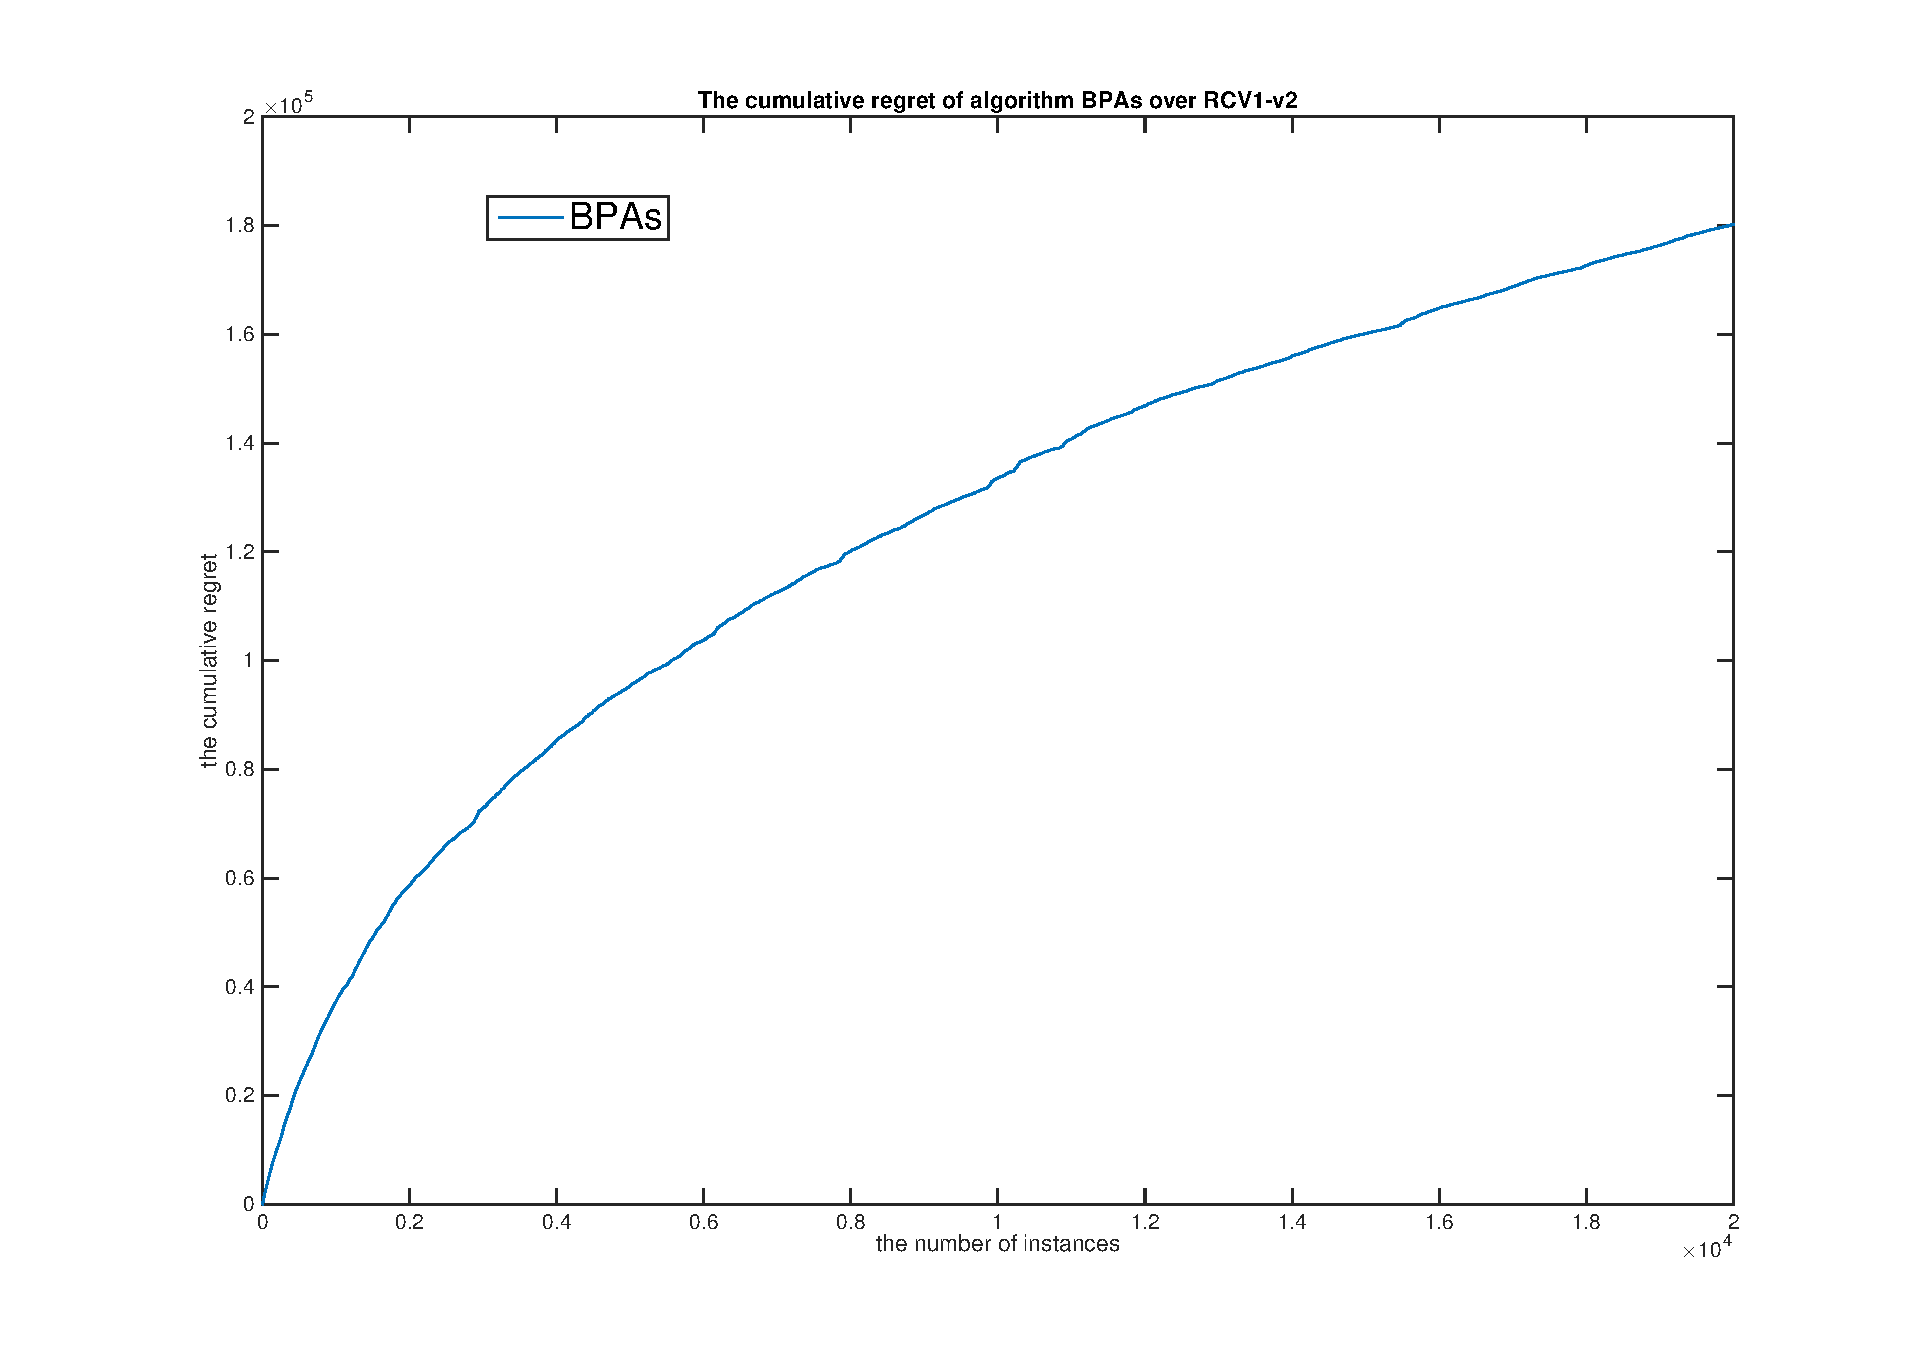
\includegraphics[scale = 0.6]{fig05/ml/regret.eps}}
\caption{The cumulative regret of algorithms on RCV1-v2}
\label{pig:regret}
\end{figure}

\begin{figure}[h!]
\vspace{.2in}
\centerline{
\includegraphics[scale = 0.6]{fig05/ml/Precision_Yeast.png}}
\caption{Precision of algorithms on Yeast}
\label{pig:PY}
\end{figure}

\begin{figure}[h!]
\vspace{.2in}
\centerline{
\includegraphics[scale = 0.6]{fig05/ml/Recall_Yeast.png}}
\caption{Recall of algorithms on Yeast}
\label{pig:RY}
\end{figure}

\begin{figure}[h!]
\vspace{.2in}
\centerline{
\includegraphics[scale = 0.6]{fig05/ml/OneError_Yeast.png}}
\caption{OneError of algorithms on Yeast}
\label{pig:OEY}
\end{figure}


\begin{figure}[h]
\vspace{.2in}
\centerline{
\includegraphics[scale = 0.6]{fig05/ml/Regret_Norm_Yeast.png}}
\caption{The cumulative regret / $\parallel{W_t}\parallel^2$ of algorithms on Yeast}
\label{pig:RegretY}
\end{figure}

\subsection{Conclusion}
\label{subsec:BPASC}
Here goes the conclusion.